\section{Introdução}

\begin{comment}
\subsection{Proposta}

    \begin{frame}{Aprendizado por Reforço}
        \begin{itemize}
        \justifying
            \item método de aprendizado por tentativa e erro, em que é utilizada a \alert{experiência} para melhorar de forma incremental a política de controle.
            \item usado para aprender tarefas de decisões sequenciais quando o modelo dinâmico do sistema é desconhecido.
            \item Uma grande área de aplicação é o seu uso na robótica em ambientes desestruturados, por exemplo, para aprender a manipular objetos novos numa tarefa de faxina em robôs domésticos.
            \item A abordagem é bem-sucedido em tarefas de curto prazo, em que o resultado da tentativa está evidente dentro de alguns (100) passos de controle. Para tarefas maiores, precisamos de alguma forma de abstração para evitar o planejamento de tarefas complexas (trazer uma bebida) em ações primitivas (atuações dos motores). Isso é chamado Aprendizado por Reforço Hierárquico.
        \end{itemize}
    \end{frame}
\end{comment}

\begin{comment}
    \begin{frame}{Proposta de Exame de Qualificação}
        \begin{itemize}
             \item  Decomposição Hierárquica busca aprender a tarefa em ações simbólicas e discretas, que podem ser sequenciadas, paralelizadas ou dispostas numa arquitetura em camadas a depender do algoritmo utilizado. O mapeamento das ações simbólicas em ações primitivas também é aprendido através de aprendizado por reforço. Os principais aspectos a serem abordados nesta proposta são:
             \begin{itemize}
                 \item Introdução;
                 \item Framework de Aprendizado por Reforço (MDP);
                 \item Métodos de Aprendizado por Reforço Hierárquico; e
                 \item Exemplos de aplicações.
             \end{itemize}
        \end{itemize}
    \end{frame}
\end{comment}

\subsection{MDP}

\begin{frame}{Framework de Aprendizado por Reforço (MDP)}
  \begin{itemize}
    \item O \alert{Markov decision process (MDP)} especifica uma configuração para o aprendizado por reforço
    \item Os MDPs permitem modelar a tomada de decisões em situações em que os resultados são em parte aleatórios e em parte sob o controle de um tomador de decisão
  \end{itemize}
  \textbf{Definição}
    \begin{enumerate}
        \item O processo de decisão de Markov é uma 4-tupla (S,A,R,T) com:
        \begin{itemize}
            \item conjunto de possíveis \alert{estados} S
            \item conjunto de possíveis \alert{ações} A
            \item \alert{função de recompensa} de valor real R
            \item \alert{probabilidades de transição} T
        \end{itemize}
        \item MDP deve cumprir as propriedades de Markov;
        \begin{itemize}
            \item os efeitos de executar uma ação em um estado depende somente do estado e não da história anterior.
        \end{itemize}
    \end{enumerate}
\end{frame}

\subsection{RL}

\begin{frame}{Reinforcement Learning}
    \begin{itemize}
    \justifying
        \item Um agente aprende ao interagir com o ambiente;
        \item Não há necessidade de pares de entradas e resultados corretos;
        \item Realimentação está restrita a um sinal de recompensa; e
        \item Imita a aprendizagem humana em ambientes reais.
    \end{itemize}
    \begin{figure}
        \centering
        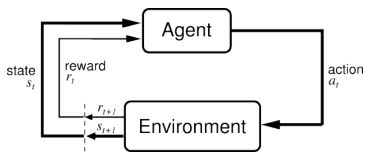
\includegraphics[width=0.7\textwidth]{img/rl.png}
        \label{fig:my_label}
    \end{figure}
\end{frame}

\begin{frame}{Reinforcement Learning}
    \textbf{Encontrar um comportamento ótimo}:
    \begin{itemize}
        \item Aprender o melhor comportamento $\pi$ baseado em ações passadas; e
        \item Maximiza a recompensa cumulativa esperada ao longo do tempo.
    \end{itemize}
    \textbf{Desafios}:
    \begin{itemize}
        \item Retroalimentação é atrasada, não instantânea; e
        \item O Agente deve aprender sobre as consequências a longo prazo de suas ações.
    \end{itemize}
    %\textbf{Ilustração}:
    %\begin{itemize}
    %    \item Visando maximizar o lucro futuro, é preciso estudar agora
    %    \item No entanto, a recompensa monetária imediata disso pode ser negativa
    %\end{itemize}
\end{frame}

\begin{frame}{Reinforcement Learning}
    Técnicas para buscar a solução ótima.\\
    \vspace{7pt}%em, ex, in, pt, pc, cm, mm, dd, cc, nd, nc, bp, sp
    Aprendizado por tentativa e erro:
    \begin{itemize}
        \item \alert{Exploração}:
        \begin{itemize}
            \item Tentar uma ação nova ou não ótima para aprender sua recompensa; e
            \item Aprender o ambiente melhor.
        \end{itemize}
        \item \alert{Explotação}:
        \begin{itemize}
            \item Usar o conhecimento já aprendido; e
            \item Isso pode não ser ótimo ainda, contribui para aprendizado conhecido/adjacente.
        \end{itemize}
    \end{itemize}
\end{frame}

\begin{frame}{Reinforcement Learning}
    Técnicas para buscar a solução ótima.\\
    \vspace{7pt}%em, ex, in, pt, pc, cm, mm, dd, cc, nd, nc, bp, sp
    Aprendizado por tentativa e erro.\\
    \vspace{7pt}%em, ex, in, pt, pc, cm, mm, dd, cc, nd, nc, bp, sp
    \textbf{Ação de Seleção $\epsilon$-Greedy} \nocite{uniFreiburgDe}:
    \begin{itemize}
        \item Escolhe entre \alert{exploração} e \alert{explotação}:
        \begin{itemize}
            \item probabilidade ($\epsilon) \rightarrow \pi(a) = rand(a)$; e
            \item com probabilidade $(1 - \epsilon) \rightarrow \pi(a) = arg \max_{a'} Q(a')$
        \end{itemize}
        \item normalmente usa-se $\epsilon = 0.1$
    \end{itemize}    
\end{frame}

\begin{comment}
    \begin{frame}{Reinforcement Learning}
        \justifying
        
        \begin{enumerate}
            \item Aprendizado livre de modelo
            \begin{itemize}
                \item Ideia: \alert{aprenda diretamente a partir de iterações} com o ambiente
                \item Somente usa experiência a partir de sequências de estados, ação e recompensas
            \end{itemize}
        \end{enumerate}
        
        \begin{enumerate}
            \item Abordagens comuns
            \begin{itemize}
                \item \textbf{Monte Carlo métodos} são simples mas tem \alert{convergência lenta}
                \item \textbf{Q-learning} é mais \alert{eficiente} devido ao aprendizado sem-política
            \end{itemize}
        \end{enumerate}
        
        \begin{enumerate}
            \item Desvantagens de aprendizado baseado em modelo
            \begin{itemize}
                \item Requer MDP, e.g. model explicíto da dinâmica no ambiente
                \item Probabilidades de transição são normalmente indisponíveis ou difíceis de definir
                \item Aprendizado baseado em modelo é, portanto, muitas vezes intratável mesmo em casos simples
            \end{itemize}
        \end{enumerate}
        
    \end{frame}
\end{comment}

\subsection{SMDP}

\begin{frame}{}
    Any MDP with fixed set of options is an SMDP.
\end{frame}



